\documentclass[titlepage,10pt,letterpaper]{article}
\usepackage[utf8]{inputenc}
\usepackage[margin=0.6in]{geometry}
\usepackage{multicol}
\usepackage{amsmath}
\usepackage{amssymb}
\usepackage{chemformula}
\usepackage{chemfig}
\usepackage{tikz}
\usepackage{enumitem}
\usepackage{graphicx}
\usepackage{booktabs}

\tikzset{
    every node/.style={font=\small},
    grid/.style={very thin, gray!40}
}

% Set uniform compact dimensions for chemfig to avoid overlaps inside multicols
\setchemfig{atom sep=1.5em, label sep=2pt, bond offset=1pt, double bond sep=2pt}

\title{2025 U.S. National Chemistry Olympiad\\National Exam Part I}
\date{}

\begin{document}

\maketitle

\begin{multicols}{2}

\begin{enumerate}[leftmargin=*]

\item Adipic acid ($M=146.15$) is prepared by the partial oxidation of cyclohexane ($M=84.16$) according to the following balanced reaction:
\[ 2\ \chemfig{*6(------)} + 5\ \ch{O2}(g) \rightarrow 2\ \chemfig{HO-(=[::60]O)-[::-60]-[::60]-[::-60]-[::60]-(=[::60]O)-[::-60]OH} + 2\ \ch{H2O}(l) \]
A sample of 25.0~g cyclohexane reacts with excess oxygen to give 33.5~g of adipic acid. What is the yield of the reaction?
\begin{enumerate}[label=(\alph*)]
    \item 38.6\%
    \item 39.9\%
    \item 48.9\%
    \item 77.2\%
\end{enumerate}

\item When a 1.000~g sample of \ch{CoCO3} is heated under vacuum, it forms 0.630~g of an oxide of cobalt. When this sample is exposed to air, it forms a second oxide of cobalt, and attains a mass of 0.675~g. What are the formulas of the first and second oxide of cobalt, respectively?
\begin{enumerate}[label=(\alph*)]
    \item \ch{CoO}, \ch{Co2O3}
    \item \ch{CoO}, \ch{Co3O4}
    \item \ch{Co2O3}, \ch{Co3O4}
    \item \ch{Co3O4}, \ch{Co2O3}
\end{enumerate}

\item A white, crystalline solid contains only the elements C, H, N, and O. Complete combustion of a 1.000~g sample gives 1.831~g \ch{CO2} ($M=44.01$) and 0.750~g \ch{H2O} ($M=18.02$). What is its molecular formula?
\begin{enumerate}[label=(\alph*)]
    \item \ch{C3H6NO}
    \item \ch{C4H4NO2}
    \item \ch{C6H12N2O2}
    \item \ch{C8H8N2O4}
\end{enumerate}

\item 10.0~mL of 0.100~M \ch{CaCl2} is mixed with 10.0~mL of 0.050~M \ch{AgNO3}. What is the concentration of chloride ion in the final solution?
\begin{enumerate}[label=(\alph*)]
    \item 0.025~M
    \item 0.075~M
    \item 0.100~M
    \item 0.200~M
\end{enumerate}

\item A metal sulfate decahydrate contains 31.48\% water by mass. What is the metal?
\begin{enumerate}[label=(\alph*)]
    \item \ch{Na}
    \item \ch{Cr}
    \item \ch{Rh}
    \item \ch{Au}
\end{enumerate}

\item Which procedures will result in a 1.000~m solution of sodium acetate?
\begin{enumerate}[label=\Roman*.]
    \item Adding 1.000~mol sodium acetate trihydrate to a 1.000-liter volumetric flask, adding deionized water to dissolve, and then filling to the mark
    \item Mixing 1.000~mol sodium hydroxide with 1.000~mol acetic acid and 1.000~kg deionized water
\end{enumerate}
\begin{enumerate}[label=(\alph*)]
    \item I only
    \item II only
    \item Both I and II
    \item Neither I nor II
\end{enumerate}

\item A white solid is either sodium carbonate or sodium sulfate. Which procedure will best distinguish between the two?
\begin{enumerate}[label=(\alph*)]
    \item Adding 1.0~M hydrochloric acid to the two solids
    \item Adding 1.0~M barium nitrate to solutions made from the two solids
    \item Adding 1.0~M potassium bromide to solutions made from the two solids
    \item Measuring the conductivity of solutions made from the two solids
\end{enumerate}

\item A colorimeter contains four LEDs. Which one would give the best results in determining the concentration of a substance that forms a blue solution?
\begin{enumerate}[label=(\alph*)]
    \item Violet (430~nm)
    \item Blue (470~nm)
    \item Green (565~nm)
    \item Red (635~nm)
\end{enumerate}

\item A student wishes to determine the number of colored dyes present in the ink of a black felt-tip marker. Which technique would be most suitable?
\begin{enumerate}[label=(\alph*)]
    \item Paper chromatography
    \item Gas chromatography
    \item Nuclear magnetic resonance spectroscopy
    \item Ultraviolet-visible spectroscopy
\end{enumerate}

\item A solution of a metal chloride gives a red flame test. Which metal is it?
\begin{enumerate}[label=(\alph*)]
    \item \ch{Na}
    \item \ch{K}
    \item \ch{Cu}
    \item \ch{Sr}
\end{enumerate}

\item Exposure of an aqueous solution of which ion to oxygen gas will cause a color change?
\begin{enumerate}[label=(\alph*)]
    \item \ch{Cr^{2+}}
    \item \ch{Cr2O7^{2-}}
    \item \ch{Fe(C2O4)3^{3-}}
    \item \ch{Fe(CN)6^{3-}}
\end{enumerate}

\item A student determines the rate constant for the reaction of iodide with hydrogen peroxide in strongly acidic solution ($\text{Rate} = k[\ch{H2O2}][\ch{I-}][\ch{H+}]$) by mixing 1.00~mL aliquots of solutions of known concentrations of potassium iodide, ascorbic acid, and hydrochloric acid with four drops of starch solution, then adding 1.00~mL of hydrogen peroxide solution and recording the time required for the solution to turn blue. A student uses half the stipulated amount of one of the solutions but does not realize it. Underdosing of which solutions will cause the value of the rate constant to be too high?
\begin{enumerate}[label=\Roman*.]
    \item Hydrochloric acid
    \item Ascorbic acid
\end{enumerate}
\begin{enumerate}[label=(\alph*)]
    \item I only
    \item II only
    \item Both I and II
    \item Neither I nor II
\end{enumerate}

\item 8.82~g of \ch{Br2} is placed in an evacuated 1.00~L flask and heated to $58.8^\circ\text{C}$, the normal boiling point of bromine. How much liquid bromine remains at equilibrium?
\begin{enumerate}[label=(\alph*)]
    \item 0.00~g
    \item 2.95~g
    \item 3.63~g
    \item 5.87~g
\end{enumerate}

\item The normal boiling point of dichloromethane (\ch{CH2Cl2}) is $40^\circ\text{C}$, while the normal boiling point of chloroform (\ch{CHCl3}) is $61^\circ\text{C}$. An increase in which type of intermolecular forces is most responsible for this increase in boiling point?
\begin{enumerate}[label=(\alph*)]
    \item London dispersion forces
    \item Dipole-dipole interactions
    \item Ion-dipole interactions
    \item Hydrogen bonding
\end{enumerate}

\item Which has the highest melting point?
\begin{enumerate}[label=(\alph*)]
    \item \ch{K2O}
    \item \ch{CaO}
    \item \ch{Cu2O}
    \item \ch{GeO2}
\end{enumerate}

\item Platinum crystallizes in a face-centered cubic unit cell. The atomic radius of platinum is 139~pm. What is the density of solid platinum?
\begin{enumerate}[label=(\alph*)]
    \item $5.33\text{ g cm}^{-3}$
    \item $7.54\text{ g cm}^{-3}$
    \item $18.6\text{ g cm}^{-3}$
    \item $21.3\text{ g cm}^{-3}$
\ postseason\end{enumerate}

\item Which statement about elemental sulfur (\ch{S8}) is correct?
\begin{center}
\begin{tikzpicture}[scale=0.032]
    \draw[->] (0,0) -- (120,0) node[right] {$T, {^\circ}\text{C}$};
    \draw[->] (0,0) -- (0,120) node[above] {$P, \text{bar}$};
    \draw (0,30) to[out=10,in=240] (40,40) to[out=60,in=240] (90,110);
    \draw (40,40) to[out=15,in=210] (70,50) to[out=30,in=180] (110,65);
    \draw (70,50) to[out=80,in=250] (90,110);
    \node at (25,80) {\scriptsize ortho.};
    \node at (65,65) {\scriptsize mono.};
    \node at (100,85) {\scriptsize liq.};
    \node at (70,20) {\scriptsize gas};
    \draw[dashed] (40,40) -- (40,0) node[below] {\tiny 95.6};
    \draw[dashed] (70,50) -- (70,0) node[below] {\tiny 119.6};
    \draw[dashed] (90,110) -- (90,0) node[below] {\tiny 154};
    \draw[dashed] (70,50) -- (0,50) node[left] {\tiny $1.8\cdot 10^{-5}$};
    \draw[dashed] (40,40) -- (0,40) node[left] {\tiny $3.8\cdot 10^{-6}$};
    \draw[dashed] (90,110) -- (0,110) node[left] {\tiny 1400};
\end{tikzpicture}
\end{center}
\begin{enumerate}[label=(\alph*)]
    \item Monoclinic sulfur sublimes at 1 bar pressure.
    \item Monoclinic sulfur is denser than orthorhombic sulfur.
    \item Monoclinic sulfur is not thermodynamically stable above $119.6^\circ\text{C}$.
    \item Monoclinic sulfur transforms exothermically into orthorhombic sulfur.
\end{enumerate}

\item The unit cell of solid fluorite, \ch{CaF2}, is shown below. Which statement about fluorite is correct?
\begin{center}
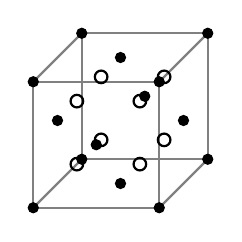
\begin{tikzpicture}[scale=1.6]
    \draw[gray, thick] (0,0,0) -- (1,0,0) -- (1,1,0) -- (0,1,0) -- cycle;
    \draw[gray, thick] (0,0,1) -- (1,0,1) -- (1,1,1) -- (0,1,1) -- cycle;
    \draw[gray, thick] (0,0,0) -- (0,0,1);
    \draw[gray, thick] (1,0,0) -- (1,0,1);
    \draw[gray, thick] (1,1,0) -- (1,1,1);
    \draw[gray, thick] (0,1,0) -- (0,1,1);
    \foreach \x in {0,1} \foreach \y in {0,1} \foreach \z in {0,1} {\draw[fill=black] (\x,\y,\z) circle (0.04);}
    \foreach \x in {0.5} \foreach \y in {0,1} \foreach \z in {0.5} {\draw[fill=black] (\x,\y,\z) circle (0.04);}
    \foreach \x in {0,1} \foreach \y in {0.5} \foreach \z in {0.5} {\draw[fill=black] (\x,\y,\z) circle (0.04);}
    \foreach \x in {0.5} \foreach \y in {0.5} \foreach \z in {0,1} {\draw[fill=black] (\x,\y,\z) circle (0.04);}
    \foreach \x in {0.25, 0.75} \foreach \y in {0.25, 0.75} \foreach \z in {0.25, 0.75} {\draw[thick] (\x,\y,\z) circle (0.05);}
\end{tikzpicture}
\end{center}
\begin{enumerate}[label=(\alph*)]
    \item Fluorite has a primitive cubic unit cell.
    \item The larger open circles represent the Ca atoms and the smaller filled circles represent the F atoms.
    \item The larger open circles nearest neighbors consist of six of the other larger open circles arranged in an octahedron.
    \item The smaller closed circles' nearest neighbors consist of eight of the larger open circles arranged in a cube.
\end{enumerate}

\end{enumerate}

\noindent\textbf{Questions 19 and 20 use the following thermodynamic data:}
\begin{center}
\small
\setlength{\tabcolsep}{3pt}
\begin{tabular}{lccc}
\toprule
Substance & $\Delta H^\circ_f, \text{kJ/mol}$ & $\Delta G^\circ_f, \text{kJ/mol}$ & $S^\circ, \text{J/mol}\cdot\text{K}$ \\
\midrule
\ch{Cl2}(g) & 0 & 0 & 223.1 \\
\ch{PCl3}(g) & $-287.0$ & $-267.8$ & 311.8 \\
\ch{PCl5}(g) & $-374.9$ & --- & 364.4 \\
\bottomrule
\end{tabular}
\end{center}

\begin{enumerate}[leftmargin=*,resume]
\item What is $K_p$ for the gas-phase reaction of \ch{PCl3} with \ch{Cl2} at 450~K?
\[ \ch{PCl3}(g) + \ch{Cl2}(g) \rightarrow \ch{PCl5}(g) \]
\begin{enumerate}[label=(\alph*)]
    \item 19.8
    \item $2.02\times 10^4$
    \item $3.17\times 10^6$
    \item $1.60\times 10^{10}$
\end{enumerate}

\item What is $\Delta G^\circ_f$ of \ch{PCl5} at 298~K?
\begin{enumerate}[label=(\alph*)]
    \item $-266.3\text{ kJ mol}^{-1}$
    \item $-304.9\text{ kJ mol}^{-1}$
    \item $-355.7\text{ kJ mol}^{-1}$
    \item $-374.9\text{ kJ mol}^{-1}$
\end{enumerate}

\item Which quantities are independent of the path taken, given the same initial and final state?
\begin{enumerate}[label=\Roman*.]
    \item The work done by the reaction of a mole of gaseous propane with excess gaseous oxygen to form carbon dioxide and water vapor at a constant pressure of 1.0 atm
    \item The heat absorbed by the expansion of a mole of carbon dioxide from a pressure of 4.0 atm to a pressure of 1.0 atm
\end{enumerate}
\begin{enumerate}[label=(\alph*)]
    \item I only
    \item II only
    \item Both I and II
    \item Neither I nor II
\end{enumerate}

\item The standard enthalpy of combustion of propene, \ch{C3H6}(g), is $-1926\text{ kJ mol}^{-1}$. Given the tabulated bond dissociation enthalpies (BDEs), what is the bond dissociation enthalpy of a C=C bond?
\[ \ch{C3H6}(g) + 4.5\ \ch{O2}(g) \rightarrow 3\ \ch{CO2}(g) + 3\ \ch{H2O}(g) \]
\begin{center}
\small
\setlength{\tabcolsep}{2pt}
\begin{tabular}{cc|cc}
\toprule
Bond & BDE, $\text{kJ/mol}$ & Bond & BDE, $\text{kJ/mol}$ \\
\midrule
C-H & 415 & C-O & 350 \\
O-H & 464 & C=O & 804 \\
O-O & 140 & C-C & 345 \\
O=O & 498 & C=C & ??? \\
\bottomrule
\end{tabular}
\end{center}
\begin{enumerate}[label=(\alph*)]
    \item $476\text{ kJ mol}^{-1}$
    \item $606\text{ kJ mol}^{-1}$
    \item $690\text{ kJ mol}^{-1}$
    \item $715\text{ kJ mol}^{-1}$
\end{enumerate}

\item Which reaction has $\Delta S^\circ > 0$?
\begin{enumerate}[label=(\alph*)]
    \item \ch{Ga}(l) $\rightarrow$ \ch{Ga}(s)
    \item \ch{C60}(s) $\rightarrow$ 60 \ch{C}(s, graphite)
    \item \ch{CaCO3}(s) $\rightarrow$ \ch{Ca^{2+}}(aq) + \ch{CO3^{2-}}(aq)
    \item \ch{NH4+}(aq) + \ch{OH-}(aq) $\rightarrow$ \ch{NH3}(aq) + \ch{H2O}(l)
\end{enumerate}

\item A sample of 10.0~g ammonium nitrate ($M=80.1$) is added to 100.0~g water in a well-insulated container. The solid and liquid are both initially at $22.0^\circ\text{C}$, and the temperature of the solution after the ammonium nitrate has dissolved is $15.1^\circ\text{C}$. What is the enthalpy of solution of ammonium nitrate? You may assume that the specific heat capacity of the solution is the same as that of pure water, $4.184\text{ J g}^{-1}\text{K}^{-1}$.
\[ \ch{NH4NO3}(s) \rightarrow \ch{NH4+}(aq) + \ch{NO3-}(aq) \]
\begin{enumerate}[label=(\alph*)]
    \item $-3.2\text{ kJ mol}^{-1}$
    \item $3.2\text{ kJ mol}^{-1}$
    \item $5.5\text{ kJ mol}^{-1}$
    \item $25\text{ kJ mol}^{-1}$
\end{enumerate}

\item The rate law for the oxidation of iodide to iodine by hydrogen peroxide in weakly acidic solution is studied by allowing the reaction to proceed in the presence of a fixed amount of sodium thiosulfate (which rapidly reduces iodine to iodide) and measuring the time to the first appearance of a blue color due to the starch-iodine complex. The following data are obtained on solutions made with the indicated volumes of reactant solutions and enough water to give a total volume of 10.0~mL. What are the reaction orders in \ch{H2O2}, \ch{I-}, and \ch{H+}?
\[ \ch{H2O2}(aq) + 2\ \ch{I-}(aq) + 2\ \ch{H+}(aq) \rightarrow \ch{I2}(aq) + 2\ \ch{H2O}(l) \]
\begin{center}
\small
\setlength{\tabcolsep}{2pt}
\begin{tabular}{cccccc}
\toprule
Run & \ch{CH3COOH}, mL & \ch{NaOH}, mL & \ch{KI}, mL & \ch{H2O2}, mL & $t$, s \\
\midrule
1 & 2.0 & 1.0 & 2.0 & 2.0 & 68.2 \\
2 & 4.0 & 1.0 & 2.0 & 2.0 & 68.9 \\
3 & 2.0 & 1.0 & 4.0 & 2.0 & 33.2 \\
4 & 2.0 & 1.0 & 2.0 & 4.0 & 32.9 \\
\bottomrule
\end{tabular}
\end{center}
\vspace{1ex}
\noindent\small
\begin{tabular}{cccc}
\toprule
& Order in \ch{H2O2} & Order in \ch{I-} & Order in \ch{H+} \\
\midrule
(A) & 0 & 1 & 1 \\
(B) & 1 & 1 & 0 \\
(C) & 1 & 1 & 1 \\
(D) & 1 & 2 & 2 \\
\bottomrule
\end{tabular}

\item The oxidation of cyanide ion to cyanate ion by hypoiodite is proposed to take place by the following mechanism. If the pH is greater than either the $pK_a$ of \ch{HOI} or of \ch{HCN}, what is the rate law?
\begin{align*}
    \ch{OI-} + \ch{H+} &\rightleftharpoons \ch{HOI} \quad \text{(fast)} \\
    \ch{CN-} + \ch{HOI} &\rightleftharpoons \ch{ICN} + \ch{OH-} \quad \text{(fast)} \\
    \ch{ICN} + \ch{OH-} &\rightarrow \ch{HOCN} + \ch{I-} \quad \text{(slow)} \\
    \ch{HOCN} + \ch{OH-} &\rightarrow \ch{OCN-} + \ch{H2O} \quad \text{(fast)}
\end{align*}
\begin{enumerate}[label=(\alph*)]
    \item $\text{Rate} = k[\ch{CN-}][\ch{OI-}]$
    \item $\text{Rate} = k[\ch{CN-}][\ch{OI-}][\ch{H+}]$
    \item $\text{Rate} = k[\ch{CN-}][\ch{OI-}][\ch{OH-}]$
    \item $\text{Rate} = k[\ch{CN-}][\ch{OI-}][\ch{OH-}]^2$
\end{enumerate}

\item $^{86}\text{Se}$ undergoes $\beta^-$ decay to $^{86}\text{Br}$ with a half-life of 14.3~s. $^{86}\text{Br}$ then undergoes $\beta^-$ decay to $^{86}\text{Kr}$, a stable product. $0.100\text{ g}\ ^{86}\text{Se}$ was placed in a sealed vessel, and the masses of all three species were recorded over time as shown below. What is the half-life of $^{86}\text{Br}$?
\begin{center}
\begin{tikzpicture}[scale=0.032]
    \draw[step=5, gray!20, very thin] (0,0) grid (100,100);
    \draw[step=10, gray!50, thin] (0,0) grid (100,100);
    \draw[->, thick] (0,0) -- (105,0) node[right] {$t \text{ (s)}$};
    \draw[->, thick] (0,0) -- (0,105) node[above] {\text{Mass (mg)}};
    \foreach \x in {0,20,40,60,80,100} \node[below] at (\x,0) {\tiny \x};
    \foreach \y in {0,20,40,60,80,100} \node[left] at (0,\y) {\tiny \y};
    \draw[thick] (0,100) to[out=-70,in=175] (20,38) to[out=-5,in=179] (50,10) to[out=0,in=180] (100,1);
    \draw[thick, dashed] (0,0) to[out=70,in=170] (25,55) to[out=-10,in=160] (40,62) to[out=-20,in=140] (100,38);
    \draw[thick, dashdotted] (0,0) to[out=5,in=200] (30,15) to[out=20,in=210] (60,42) to[out=30,in=205] (100,61);
\end{tikzpicture}
\end{center}
\begin{enumerate}[label=(a)]
    \item 55~s
    \item 70.~s
    \item 85~s
    \item It cannot be determined from the information given.
\end{enumerate}

\item A reactant R undergoes independent, irreversible first-order reactions to form two products, X and Y. The reaction to form X has an activation energy that is $20.0\text{ kJ mol}^{-1}$ higher than the activation energy of the reaction to form Y. At $50.0^\circ\text{C}$ the yield of X is 50.0\%. What is the yield of X at $70.0^\circ\text{C}$?
\begin{enumerate}[label=(\alph*)]
    \item 32.5\%
    \item 39.4\%
    \item 60.6\%
    \item 77.0\%
\end{enumerate}

\item The reaction of \textit{tert}-butyl chloride, \chemfig{-[::30](-[::60])(-[::-60])-Cl}, with azide ion takes place via a carbocation intermediate \chemfig{-[::30](-[::60])(-[::-60])-[::0]^{+}} as shown on the reaction coordinate diagram below. The reaction proceeds faster in polar solvents. Which dashed line best represents the profile in a less polar option?
\begin{center}
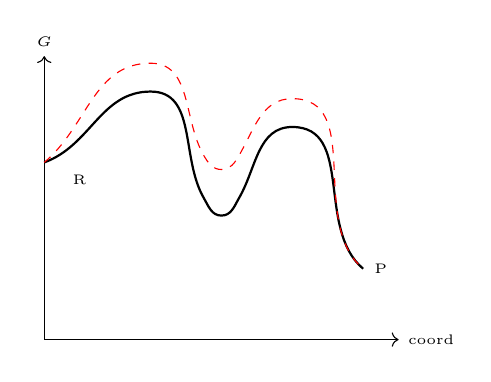
\begin{tikzpicture}[scale=0.45]
    \draw[->] (0,0) -- (10,0) node[right] {\tiny coord};
    \draw[->] (0,0) -- (0,8) node[above] {\tiny $G$};
    \draw[thick] (0,5) to[out=20,in=180] (3,7) to[out=0,in=120] (4.5,4) to[out=300,in=180] (5,3.5) to[out=0,in=240] (5.5,4) to[out=60,in=180] (7,6) to[out=0,in=140] (9,2);
    \draw[dashed, red] (0,5) to[out=40,in=180] (3,7.8) to[out=0,in=120] (4.5,5.2) to[out=300,in=180] (5,4.8) to[out=0,in=240] (5.5,5.2) to[out=60,in=180] (7,6.8) to[out=0,in=140] (9,2);
    \node at (1,4.5) {\tiny R};
    \node at (9.5,2) {\tiny P};
\end{tikzpicture}
\end{center}
\begin{enumerate}[label=(\alph*)]
    \item A
    \item B
    \item C
    \item D
\end{enumerate}

\item The reaction of hydroxide ion with methyl iodide takes place in a single elementary step. The reaction is faster when the carbon-12 isotope is present than when carbon-14 is present ($k_{12}/k_{14} = 1.088$). What is the principal reason for the difference in rates?
\[ \chemfig{-I} + \ch{OH-} \rightarrow \chemfig{-OH} + \ch{I-} \]
\begin{enumerate}[label=(\alph*)]
    \item The carbon nucleus is less stable in $^{14}\ch{CH3I}$.
    \item The vibrational energies are lower in $^{14}\ch{CH3I}$.
    \item The molecule is less sterically hindered in $^{14}\ch{CH3I}$.
    \item The carbon-iodine bond dissociation enthalpy is smaller in $^{14}\ch{CH3I}$.
\end{enumerate}

\item Given the equilibrium constants:
\begin{align*}
    \ch{Ag+}(aq) + \ch{Cl-}(aq) &\rightleftharpoons \ch{AgCl}(s) \quad &K_1 \\
    2\ \ch{Ag+}(aq) + \ch{CrO4^{2-}}(aq) &\rightleftharpoons \ch{Ag2CrO4}(s) \quad &K_2
\end{alignmined}
What is the equilibrium constant for the following reaction?
\[ 2\ \ch{AgCl}(s) + \ch{CrO4^{2-}}(aq) \rightleftharpoons \ch{Ag2CrO4}(s) + 2\ \ch{Cl-}(aq) \]
\begin{enumerate}[label=(\alph*)]
    \item $\frac{K_1}{K_2}$
    \item $\frac{K_1}{K_2^2}$
    \item $\frac{K_2^2}{K_1}$
    \item $\frac{K_2}{K_1^2}$
\end{enumerate}

\item A solution of allylamine, \chemfig{H_2N-[::-30]-[::60]=_[::-60]}, is 3.61\% ionized and has a $\text{pH} = 11.12$. What is the $pK_a$ of the allylammonium ion?
\begin{enumerate}[label=(\alph*)]
    \item 3.77
    \item 9.69
    \item 10.23
    \item 12.56
\end{enumerate}

\item A solution of formic acid, \chemfig{H-(=[::60]O)-[::-60]OH}, is titrated with 0.1000~M \ch{NaOH}. At the point where 15.0~mL of \ch{NaOH} have been added, what are the relative concentrations of Formic acid, Formate, and \ch{Na+}?
\begin{enumerate}[label=(\alph*)]
    \item $[\text{Formate}^-] > [\ch{Na+}] > [\text{Formic acid}]$
    \item $[\text{Na}^+] > [\text{Formate}^-] > [\text{Formic acid}]$
    \item $[\text{Formic acid}] > [\ch{Na+}] > [\text{Formate}^-]$
    \item $[\text{Formic acid}] > [\text{Formate}^-] > [\ch{Na+}]$
\end{enumerate}

\item At high temperatures, solid calcium carbonate is in equilibrium with solid calcium oxide and carbon dioxide gas.
\[ \ch{CaCO3}(s) \rightleftharpoons \ch{CaO}(s) + \ch{CO2}(g) \]
Into an evacuated 30.0~L chamber maintained at 1200~K is introduced 3.0~g solid \ch{CaCO3}. After equilibration, the pressure is 0.10~bar. What will the total pressure be if an additional 3.0~g \ch{CaCO3} is added?
\begin{enumerate}[label=(\alph*)]
    \item 0.10 bar
    \item 0.14 bar
    \item 0.20 bar
    \item It cannot be determined from the information given.
\end{enumerate}

\item At a certain temperature, the reaction below has $K_p = 3.75$. Initially, all four gases are in a rigid container, each with a partial pressure of 0.60~bar. What will the partial pressure of \ch{SO2}(g) be once the system achieves equilibrium?
\[ \ch{SO2}(g) + \ch{NO2}(g) \rightleftharpoons \ch{SO3}(g) + \ch{NO}(g) \]
\begin{enumerate}[label=(\alph*)]
    \item 0.19 bar
    \item 0.25 bar
    \item 0.35 bar
    \item 0.41 bar
\end{enumerate}

\item Cadmium iodate, \ch{Cd(IO3)2}, has $K_{sp} = 2.5\times 10^{-8}$. Iodide ion forms a complex ion \ch{CdI4^{2-}} with $K_f = 1.3\times 10^6$. What is the minimum amount of iodide ion that would need to be added to dissolve 0.100~mol \ch{Cd(IO3)2} in 1.00~L of solution?
\begin{enumerate}[label=(\alph*)]
    \item 0.40 mol
    \item 0.59 mol
    \item 0.62 mol
    \item 0.99 mol
\end{enumerate}

\item What is the average oxidation state of molybdenum in the phosphomolybdate ion \ch{PMo12O40^{3-}}?
\begin{enumerate}[label=(\alph*)]
    \item +6.00
    \item +6.17
    \item +6.42
    \item +6.50
\end{enumerate}

\item For a voltaic cell $\ch{Zn}|\ch{Zn^{2+}}(1.0\text{ M})||\ch{Ag+}(1.0\text{ M})|\ch{Ag}$, which is correct?
\begin{enumerate}[label=(\alph*)]
    \item The zinc electrode is the anode.
    \item The concentration of \ch{Ag+} increases as the cell operates.
    \item The mass of the zinc electrode increases as the cell operates.
    \item Electrons flow through the external circuit from the silver electrode to the zinc electrode.
\end{enumerate}

\item A 1.000~g sample of a gold compound is electrolyzed exhaustively to deposit all the gold present on the cathode. This requires 4700~s of electrolysis with a constant current of 0.130~A. What is the compound?
\begin{enumerate}[label=(\alph*)]
    \item \ch{LiAuCl2} ($M=274.8$)
    \item \ch{LiAuCl4} ($M=345.7$)
    \item \ch{CsAuCl2} ($M=400.8$)
    \item \ch{CsAuCl4} ($M=471.7$)
\end{enumerate}

\item Which factors contribute to inefficiencies in silicon-based photovoltaic devices in harvesting the energy of light from the sun?
\begin{enumerate}[label=\Roman*.]
    \item Photons with energies less than the band gap of silicon are not absorbed by the device.
    \item Energy is lost as heat when photons with energies greater than the band gap of silicon are absorbed by the device.
\end{enumerate}
\begin{enumerate}[label=(\alph*)]
    \item I only
    \item II only
    \item Both I and II
    \item Neither I nor II
\end{enumerate}

\item The standard reduction potential $E^\circ$ for the reduction of permanganate to manganese(II) in acidic solution is 1.51~V at 298~K. What is the value of E for the half-reaction at 298~K at the given concentrations?
\[ \ch{MnO4-}(aq, 0.0100\text{ M}) + 8\ \ch{H+}(aq, 0.200\text{ M}) + 5\ \ch{e-} \rightarrow \ch{Mn^{2+}}(aq, 0.0200\text{ M}) + 4\ \ch{H2O}(l) \]
\begin{enumerate}[label=(\alph*)]
    \item 1.16 V
    \item 1.44 V
    \item 1.50 V
    \item 1.51 V
\end{enumerate}

\item What is the standard reduction potential $E^\circ$ for the reduction of hydrogen selenate to hydrogen selenide?
\[ \ch{HSeO4-}(aq) + 9\ \ch{H+}(aq) + 8\ \ch{e-} \rightarrow \ch{H2Se}(aq) + 4\ \ch{H2O}(l) \]
\begin{center}
\small
\setlength{\tabcolsep}{2pt}
\begin{tabular}{lc}
\toprule
Half-reaction & $E^\circ$, V \\
\midrule
\ch{HSeO4-}(aq) + 3\ \ch{H+} + 2\ \ch{e-} $\rightarrow$ \ch{H2SeO3} & 1.15 \\
\ch{H2SeO3}(aq) + 4\ \ch{H+} + 4\ \ch{e-} $\rightarrow$ \ch{Se}(s) & 0.74 \\
\ch{Se}(s) + 2\ \ch{H+} + 2\ \ch{e-} $\rightarrow$ \ch{H2Se}(aq) & $-0.11$ \\
\bottomrule
\end{tabular}
\end{center}
\begin{enumerate}[label=(\alph*)]
    \item 0.30 V
    \item 0.63 V
    \item 0.71 V
    \item 1.78 V
\end{enumerate}

\item In what group is the atom with the following ionization energies?
\begin{center}
\small
\begin{tabular}{cccc}
\toprule
$IE_1$ & $IE_2$ & $IE_3$ & $IE_4$ \\
\midrule
738 & 1450 & 7730 & 10500 \\
\bottomrule
\end{tabular}
\end{center}
\begin{enumerate}[label=(\alph*)]
    \item Group 1
    \item Group 2
    \item Group 3
    \item Group 13
\end{enumerate}

\item In a ground-state gas-phase Sb atom, how many electrons have the quantum numbers $n=5, l=1, m_l=0$?
\begin{enumerate}[label=(\alph*)]
    \item 1
    \item 2
    \item 3
    \item 6
\end{enumerate}

\item Two atomic orbitals have the same number of radial nodes and the same magnetic quantum number $m$. Which other quantum numbers must these orbitals have in common?
\begin{enumerate}[label=\Roman*.]
    \item The principal quantum number $n$
    \item The angular momentum quantum number $l$
\end{enumerate}
\begin{enumerate}[label=(\alph*)]
    \item I only
    \item II only
    \item Both I and II
    \item Neither I nor II
\end{enumerate}

\item The p block elements in the third row of the periodic table release more energy when an electron is added to the gas phase atoms than do their lighter congeners. Which is the best explanation?
\begin{enumerate}[label=(\alph*)]
    \item Heavier elements have more protons and greater electrostatic attraction.
    \item Heavier elements have more neutrons and greater gravitational attraction.
    \item The 3p orbitals are larger and have less electron-electron repulsion.
    \item The 3p orbitals have more nodes and accept electrons at lower energy.
\end{enumerate}

\item Which elements are closest in electronegativity?
\begin{enumerate}[label=(\alph*)]
    \item C and Al
    \item O and Cl
    \item N and P
    \item P and As
\end{enumerate}

\item By what mode does $^{212}\text{Po}$ undergo radioactive decay?
\begin{enumerate}[label=(\alph*)]
    \item $\alpha$ decay
    \item $\beta^-$ decay
    \item Positron emission
    \item Spontaneous fission
\end{enumerate}

\item Which species has a square planar geometry?
\begin{enumerate}[label=(\alph*)]
    \item \ch{BH4-}
    \item \ch{SF4}
    \item \ch{ZnCl4^{2-}}
    \item \ch{AuCl4-}
\end{enumerate}

\item Which isomer of CNO is most stable?
\begin{enumerate}[label=(\alph*)]
    \item Linear CNO
    \item Linear NCO
    \item Linear CON
    \item Cyclic CNO
\end{enumerate}

\item How many stereoisomers of octahedral \ch{Co(en)2Cl2+} are possible?
\begin{enumerate}[label=(\alph*)]
    \item 1
    \item 2
    \item 3
    \item 4
\end{enumerate}

\item Which statement most accurately describes the bonding in the acetyl cation, \chemfig{-[::30]C\equiv O^{+}}?
\begin{enumerate}[label=(\alph*)]
    \item The species has five $\sigma$ bonds and two $\pi$ bonds.
    \item The carbon-oxygen bond has a bond order of 2.
    \item The carbon bonded to oxygen has a bent geometry.
    \item The most significant resonance structure has a formal positive charge on carbon.
\end{enumerate}

\item Which of the labeled protons in ascorbic acid is the most acidic?
\begin{center}
\chemfig{O=C-C(-O-[::30]H_D)=C(-O-[::-30]H_C)-CH(-CH(-[4]OH)-[0]-[:-30]OH)-O-1}
\end{center}
\begin{enumerate}[label=(\alph*)]
    \item A
    \item B
    \item C
    \item D
\end{enumerate}

\item Which statements about the gas-phase molecule NF are correct?
\begin{enumerate}[label=\Roman*.]
    \item It has two unpaired electrons in its lowest-energy state.
    \item It has a smaller ionization energy than atomic N.
\end{enumerate}
\begin{enumerate}[label=(\alph*)]
    \item I only
    \item II only
    \item Both I and II
    \item Neither I nor II
\end{enumerate}

\item How many stable isomers of \ch{C4H8} are there?
\begin{enumerate}[label=(\alph*)]
    \item 3
    \item 4
    \item 5
    \item 6
\end{enumerate}

\item Which compound absorbs infrared radiation strongly at $1715\text{ cm}^{-1}$?
\begin{center}
\small
\begin{tabular}{cc}
(A) \chemfig{*6(------)} & (B) \chemfig{*6(---(=O)---)} \\
(C) \chemfig{*6(---(-OH)---)} & (D) \chemfig{*6(---(=)---)}
\end{tabular}
\end{center}
\begin{enumerate}[label=(\alph*)]
    \item A
    \item B
    \item C
    \item D
\end{enumerate}

\item An unknown alcohol is thought to be either 2-pentanol or 3-pentanol. Which instrumental method would most effectively distinguish between these two possibilities?
\begin{enumerate}[label=(\alph*)]
    \item Mass spectrometry
    \item Infrared spectroscopy
    \item Ultraviolet spectroscopy
    \item $^{13}\text{C}$ NMR spectroscopy
\end{enumerate}

\item Gutta percha is a naturally occurring polymer built from which monomeric building block?
\begin{center}
\chemfig{-[::-30]-[::60](-[::60])=_[::-60]-[::60]-}
\end{center}
\begin{enumerate}[label=(\alph*)]
    \item 2-methyl-1-butene
    \item 3-methyl-1-butene
    \item 2-methyl-1,3-butadiene
    \item 3-methyl-1,2-butadiene
\end{enumerate}

\item In the presence of which catalysts will the two esters below hydrolyze at different rates from each other?
\begin{center}
\small
\begin{tabular}{cc}
\chemfig{*6(=-=-=-)(-[0]=O)-[2]O-[0]-[:-30]} & \chemfig{[:-30]--[0]O-[2](=[0]O)-[4]*6(=-=-=-)}
\end{tabular}
\end{center}
\begin{enumerate}[label=\Roman*.]
    \item \ch{H2SO4}
    \item Pig liver esterase
\end{enumerate}
\begin{enumerate}[label=(\alph*)]
    \item I only
    \item II only
    \item Both I and II
    \item Neither I nor II
\end{enumerate}

\item Which structure does not readily produce D-glucose when dissolved in acidic solution?
\begin{center}
\small
\begin{tabular}{cc}
(A) \chemfig{H-(=[::60]O)-[::-60](-[::60]OH)-[::-60](-[::-60]OH)-[::-60](-[::60]OH)-[::-60](-[::-60]OH)-[::-60]-OH} & (B) Haworth formula
\end{tabular}
\end{center}
\begin{enumerate}[label=(\alph*)]
    \item A
    \item B
    \item C
    \item D
\end{enumerate}

\end{enumerate}

\end{multicols}
\end{document}